\documentclass[a4paper, 11pt]{article}
\usepackage[utf8]{inputenc}
\usepackage{vhistory}
\usepackage{amsfonts}
\usepackage{mathtools}
\usepackage{float}
\usepackage{blindtext}
\usepackage[inline]{enumitem}
\usepackage{xcolor}
\usepackage{amsmath, amssymb, lmodern}
\usepackage{array}
\usepackage{listings}
\usepackage{svg}
\usepackage{color}
\usepackage{booktabs}
\usepackage{caption}
\usepackage{varioref}
\usepackage{hyperref} 
\usepackage[ruled,vlined]{algorithm2e}
\usepackage[section]{placeins}
\usepackage{comment} % enables the use of multi-line comments (\ifx \fi) 
\usepackage{graphicx}
\usepackage{lipsum} %This package just generates Lorem Ipsum filler text. 
\usepackage{fullpage} % changes the margin
\usepackage{cleveref}
\definecolor{dkgreen}{rgb}{0,0.6,0}
\definecolor{gray}{rgb}{0.5,0.5,0.5}
\definecolor{mauve}{rgb}{0.58,0,0.82}
%Includes "References" in the table of contents
\usepackage[nottoc]{tocbibind}

\DeclareMathOperator*{\argmax}{argmax} % thin space, limits underneath in displays

\newenvironment{conditions}
{\par\vspace{\abovedisplayskip}\noindent\begin{tabular}{>{$}l<{$} @{${}={}$} l}}
	{\end{tabular}\par\vspace{\belowdisplayskip}}

\renewcommand{\lstlistingname}{Algorithm}% Listing -> Algorithm
\renewcommand{\lstlistlistingname}{List of \lstlistingname s}% List of Listings -> List of Algorithms
\crefname{listing}{algorithm}{algorithms}  
\Crefname{listing}{Algorithm}{Algorithms}
\floatname{algorithm}{Procedure}

\lstset{frame=tb,
	language=Python,
	aboveskip=3mm,
	belowskip=3mm,
	showstringspaces=false,
	columns=flexible,
	basicstyle={\small\ttfamily},
	numbers=left,
	numberstyle=\tiny\color{gray},
	keywordstyle=\color{blue},
	commentstyle=\color{dkgreen},
	stringstyle=\color{mauve},
	breaklines=true,
	breakatwhitespace=true,
	tabsize=3,
	inputencoding=latin1
}

%\setlength{\belowcaptionskip}{-10pt}
\makeatletter
\renewcommand{\paragraph}{%
	\@startsection{paragraph}{4}%
	{\z@}{1.0ex \@plus 1ex \@minus .2ex}{-1em}%
	{\normalfont\normalsize\bfseries}%
}
\makeatother

\usepackage{pgfplots}
\usepackage{tikz}
\usepackage{varwidth}
\usepgfplotslibrary{fillbetween}
\usetikzlibrary{calc,trees,positioning,arrows,chains,shapes.geometric,%
	decorations.pathreplacing,decorations.pathmorphing,shapes,%
	matrix,shapes.symbols}

\tikzstyle{object} = [rectangle, rounded corners, minimum width=3cm, minimum height=1cm,text centered, draw=white]
\tikzstyle{element} = [rectangle, rounded corners, minimum width=3cm, minimum height=1cm,text centered, draw=black]
\tikzstyle{xor} = [diamond, minimum width=1cm, minimum height=1cm, text centered, draw=black]
\tikzstyle{arrow} = [thick,->,>=stealth]

\pgfplotsset{width=\textwidth, height=\textheight*0.33,compat=newest}

\definecolor{train_color_1}{HTML}{8b402a}
\definecolor{train_color_2}{HTML}{e45e2d}
\definecolor{train_color_3}{HTML}{ef9c49}
\definecolor{train_color_4}{HTML}{fdea6f}

\definecolor{test_color_1}{HTML}{192574}
\definecolor{test_color_2}{HTML}{2e62a1}
\definecolor{test_color_3}{HTML}{43a7cb}
\definecolor{test_color_4}{HTML}{9ed5cd}

\pgfplotscreateplotcyclelist{train}{
	semithick,train_color_1\\%
	semithick,train_color_2\\%
	semithick,train_color_3\\%
	semithick,train_color_4\\%
}

\pgfplotscreateplotcyclelist{test}{
	semithick,test_color_1\\%
	semithick,test_color_2\\%
	semithick,test_color_3\\%
	semithick,test_color_4\\%
}



\captionsetup[figure]{skip=0pt}


\begin{document}
	%Header-Make sure you update this information!!!!
	\noindent
	\large\textbf{A Study of Reinforcement Learning} \hfill \textbf{Report SAC} \\
	\normalsize Prof. Pietro Michiardi - Eurecom \hfill   Piero Macaluso\\
	\normalsize Prof. Elena Baralis - Politecnico di Torino  \hfill Version: \vhCurrentVersion \space from \vhCurrentDate
	
	\tableofcontents
	\newpage
	\begin{versionhistory}
		\vhEntry{1.0}{April, 26 2019}{PM}{- Created.
			
			- Added SAC description and implementation.
			
			- Added Environments Description
			
			- Added Uniform/Prioritized Replay implementation and simulation.
		}
		%\vhEntry{1.1}{23.01.04}{DP|JPW}{correction}
		%\vhEntry{1.2}{03.02.04}{DP|JPW}{revised after review}
	\end{versionhistory}
	\newpage
	
	\section{Introduction} \label{introduction}
	
	After the analysis of \textbf{Deep Deterministic Policy Gradient (DDPG)} \cite{lillicrap2015continuous}, I decided to explore other algorithms. \textbf{Soft Actor-Critic (SAC)} \cite{haarnoja2018soft} \cite{haarnoja2018alg} is one of the algorithms that intrigued me because of the promises of its discoverers: higher and more stable performance than DDPG, stochastic framework and less parameter to tune.
	
	As will be clear later, the algorithm fully met the expectations.
	
	The aim of this report is to show a background of the algorithm, the performances obtained, a comparison with the performance of DDPG and possible future developments.
	
	\section{Soft Actor-Critic} \label{sac}
	\subsection{Application Field}
	% TODO: Check this

	SAC combines the off-policy actor-critic setup with a \textbf{stochastic policy (actor)}, devising a bridge between stochastic policy optimization and DDPG-style approaches.
	
	As DDPG, SAC can be applied to situations characterized by the presence of a continuous action spaces and it is a \textbf{Model-Free}, \textbf{Off-Policy} and \textbf{Actor-Critic} algorithm.
	
	SAC algorithm is able to overcome some of the problems of DDPG.
	The latter can achieve great performance, but the interaction between the deterministic actor network and the Q-function makes it difficult to stabilize and brittle with respect to hyper-parameters and other kinds of tuning. The learned Q-function begins to dramatically overestimate Q-values, which then leads to the policy breaking, because it exploits the errors in the Q-function.
	
	For this reason, SAC exploits \textbf{Clipped Double-Q Learning} used also by \textbf{Twin Delayed DDPG (TD3)}. It learns two Q-functions instead of one, and uses the smaller of the two Q-values to form the targets in the Bellman error loss functions.
	
	Another feature of SAC is \textbf{entropy regularization}. The policy is trained to maximize a trade-off between expected return and entropy, a measure of randomness in the policy. This is strongly related to the exploration-exploitation trade-off: increasing entropy results in more exploration, which can accelerate learning later on, but it can also prevent the policy from prematurely converging to a bad local optimum.
	
	\subsection{Key Points}
	\subsubsection{Reinforcement Learning Notation}
	The Reinforcement Learning Setup is the standard one. The problem can be defined as policy search in a Markov decision process (MDP), defined by a tuple $(\mathcal{S}, \mathcal{A}, p, r)$. The state space $\mathcal{S}$ and action space $\mathcal{A}$ are continuous and the state transition probability $p : \mathcal{S} \times \mathcal{S} \times \mathcal{A} \rightarrow [0,\infty)$ represents the probability density of the next state $s_{t+1} \in \mathcal{S}$ given the current state $s_t \in \mathcal{S}$ and action $a_t \in \mathcal{A}$. The environment emits a reward $r: \mathcal{S} \times \mathcal{A} \rightarrow [r_{\min}, r_{\max}]$ on each transition. $\rho_\pi(s_t)$ and $\rho_\pi(s_t, a_t)$ denote the state and state-action marginals of the trajectory ($\tau$) distribution induced by a policy $\pi(a_t|s_t)$.
	
	\subsubsection{Entropy-Regularized Reinforcement Learning}
	
	\textbf{Entropy} is the average rate at which information is produced by a stochastic source of data. It is, in simple terms, a quantity which describes how random a random variable is. 
	The motivation behind the use of entropy is that when the data source produces a low-probability value (rare), the event carries \textbf{more \textit{information}} than when the source data produces a high-probability value.
	
	Let $x$ be a random variable with probability mass or density function $P$. The entropy $\mathcal{H}$ of $x$ is computed from its distribution $P$ according to
	
	\begin{equation} \label{eq1:entropy}
	\mathcal{H}(P) = \mathbb{E}_{x \sim P} [- \log P(x)]
	\end{equation}.
	
	In \textbf{entropy-regularized reinforcement learning} the standard objective is generalized by augmenting it with entropy. The agent gets a bonus reward at each time step proportional to the entropy of the policy at that timestep. Assuming an infinite-horizon discounted setting, this changes the RL problem to:
	\begin{equation} \label{eq2:entropy_return}
		\pi^* = \arg \max_{\pi} \mathbb{E}_{\tau \sim \pi}\Bigg[\sum_{t=0}^{\infty} \gamma^t \bigg(R(s_t, a_t, s_{t+1}) + \alpha \mathcal{H}(\pi(\cdot|s_t))\bigg)\Bigg]
	\end{equation}	
	
	where $\alpha > 0$ is the temperature parameter that determines the relative importance of the entropy term controlling the stochasticity of the optimal policy. It is clear that the standard maximum expected return can be retrieved in the limit as $\alpha \rightarrow 0$.
	
	From \vref{eq2:entropy_return} we can derive \textbf{state-value function} $V^\pi(s)$ and \textbf{action-value function} $Q^\pi(s,a)$:
	
	\begin{equation} \label{eq3:state_value}
	V^\pi(s) = \mathbb{E}_{\tau \sim \pi}\Bigg[\sum_{t=0}^{\infty} \gamma^t \bigg(R(s_t, a_t, s_{t+1}) + \alpha \mathcal{H}(\pi(\cdot|s_t))\bigg)\bigg|s_0 = s\Bigg]
	\end{equation}	
	
	\begin{equation} \label{eq4:action_value}
	Q^\pi(s,a) = \mathbb{E}_{\tau \sim \pi}\Bigg[\sum_{t=0}^{\infty} \gamma^t R(s_t, a_t, s_{t+1}) + \alpha \sum_{t=1}^{\infty} \gamma^t \mathcal{H}(\pi(\cdot|s_t))\bigg|s_0 = s, a_0 =a\Bigg]
	\end{equation}	
	
	From these equations is possible to derive the connection between state-value and action-value function given by
	\begin{equation} \label{eq5:q_v_relation}
	V^\pi(s) = \mathbb{E}_{a\sim\pi}[Q^\pi(s,a)] + \alpha \mathcal{H}(\pi(\cdot|s))
	\end{equation}
	
	and the \textbf{Bellman equation} given by

	\begin{align} 	\label{eq6:bellman}
	Q^\pi(s,a) &= \mathbb{E}_{s'\sim P, a'\sim\pi}[R(s,a,s') + \gamma(Q^\pi(s',a') + \alpha \mathcal{H}(\pi(\cdot|s')))]\\
	&= \mathbb{E}_{s'\sim P}[R(s,a,s') + \gamma V^\pi(s')]
	\end{align}
	
	\subsubsection{Learning Equations}
	SAC algorithm learns a \textbf{policy} $\pi_\theta$, two Q-functions $Q_{\phi_1}$,  $Q_{\phi_2}$.
	
	The state-value function is emplicitly parametrized through the soft Q-function parameters and the connection is given by:
	
	\begin{align}
	V^{\pi}(s) &= \mathbb{E}_{a \sim \pi}[Q^{\pi}(s,a)] + \alpha \mathcal{H} \left(\pi(\cdot|s)\right) \\
	&= \mathbb{E}_{a \sim \pi}[Q^{\pi}(s,a) - \alpha \log \pi(a|s)] \\
	& \approx Q^{\pi}(s,\tilde{a}) - \alpha \log \pi(\tilde{a}|s), \;\;\;\;\; \tilde{a} \sim \pi(\cdot|s).	
	\end{align}
	
	In \cite{haarnoja2018soft} a function approximator for this function was introduced, but later \cite{haarnoja2018alg} the authors found it to be unnecessary.
	
	\paragraph{Learning Q}The Q-functions are learned by Mean Squared Bellman Error (MSBE) minimization, using a target value network to form the Bellman backups. They both use the same target and have loss functions:
	
	\begin{equation} \label{eq11:lossQ}
	L(\phi_i, {\mathcal D}) = \mathbb{E}_{(s_t,a_t,r_t,s_{t+1},d_t) \sim \mathcal D}\left[ \Bigg( Q_{\phi_i}(s_t,a_t) - \left(r_t + \gamma (1 - d_t) V_{\bar{\phi_i}}(s_{t+1}) \right) \Bigg)^2 \right].
	\end{equation}
	where
	\begin{equation}
	V_{\bar{\phi}}(s_{t+1}) = \min_{i=1,2}Q_{\bar{\phi}_i}(s_{t+1},a_{t+1}) - \alpha \log \pi_\theta(a_{t+1}|s_{t+1}), \;\;\;\;\; a_{t+1} \sim \pi_\theta(\cdot|s_{t+1})
	\end{equation}
	
	
	The target value network, like the target networks in DDPG, is obtained by polyak averaging the value network parameters over the course of training.
	
	
	\paragraph{Learning the Policy} The policy should act to maximize the expected future return plus expected future entropy, for each state. That is, it should maximize $V^{\pi}(s)$, which can be expanded out (as before) into
			\begin{equation}
	E_{a \sim \pi}[Q^{\pi}(s,a) - \alpha \log \pi(a|s)]
			\end{equation}
	The optimization of the policy makes use of the reparameterization trick, in which a sample from $\pi_{\theta}(\cdot|s)$ is drawn by computing a deterministic function of state, policy parameters, and independent noise. To illustrate: following the authors of the SAC paper, we use a squashed Gaussian policy, which means that samples are obtained according to
			\begin{equation}
	\tilde{a}_{\theta}(s, \xi) = \tanh\left( \mu_{\theta}(s) + \sigma_{\theta}(s) \odot \xi \right), \;\;\;\;\; \xi \sim \mathcal{N}(0, I).
			\end{equation}
			
	It is possible to rewrite the expectation over actions (pain point: the distribution depends on the policy parameters) into an expectation over noise (the distribution now has no dependence on parameters) thanks to the reparameterization trick:
	
				\begin{equation}
	\mathbb{E}_{a \sim \pi_{\theta}}[{Q^{\pi_{\theta}}(s,a) - \alpha \log \pi_{\theta}(a|s)}] = \mathbb{E}_{\xi \sim \mathcal{N}}[{Q^{\pi_{\theta}}(s,\tilde{a}_{\theta}(s,\xi)) - \alpha \log \pi_{\theta}(\tilde{a}_{\theta}(s,\xi)|s)}]
				\end{equation}
				
	To get the policy loss, the final step is to substitute $Q^{\pi_{\theta}}$ with one of our function approximators. As suggested from the authors of \cite{haarnoja2018alg}, $\min_{i=1,2}Q_{\phi_i}(s_t, \tilde{a}_{\theta}(s, \xi))$ is used. The policy is thus optimized according to
					\begin{equation} \label{eq16:policy_opt}
	\max_{\theta} \mathbb{E}_{s \sim \mathcal{D}, \xi \sim \mathcal{N}}[{\alpha \log \pi_{\theta}(\tilde{a}_{\theta}(s,\xi)|s) - \min_{i=1,2}Q_{\phi_i}(s_t, \tilde{a}_{\theta}(s, \xi)) }],
					\end{equation}
	which is almost the same as the DDPG and TD3 policy optimization, except for the stochasticity and entropy term.
	
	
	The implementation of these updates can be found in \vref{lst:update}.
	\lstinputlisting[float,linerange={108-152},firstnumber=108,label={lst:update},caption={Update Phase SAC}]{code/AgentSAC.py}

	
	
	\subsubsection{Replay Buffers} Most optimization algorithms assume that the samples are \textbf{independently and identically distributed (i.i.d)}, but data produced sequentially exploring the environment can not satisfy this assumption. To solve this problem, a Replay Buffer can be used: it is a set $\mathcal D$ of $N$ recent experiences $(s_t, a_t, r_t, s_{t+1}, d_t)$ from which the algorithm will randomly sample a subset of $M\ll N$ experiences (mini-batch) at each iteration.
	
	The replay buffer should be large enough to contain a wide range of experiences in order to have stable algorithm behavior, but it may not always be good to keep everything. Using only the very-most recent data leads to overfitting, while using too much experience may slow down the learning process.
	
	\subsubsection{Target Networks} 
	\begin{figure}[!h]
		\begin{center}
			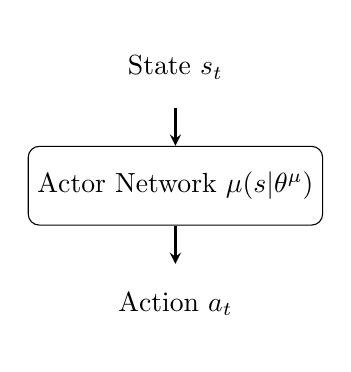
\begin{tikzpicture}
			[node distance=1.5cm]
			\node[object] (state)  {State $s_t$ };
			\node[element, below of=state] (localActor){ Actor Network $\mu(s|\theta^\mu)$};
			\node[object, below of=localActor] (action){ Action $a_t$};
			
			\draw[arrow] (state) -- (localActor);
			\draw[arrow] (localActor) -- (action);
			\end{tikzpicture}
			\begin{tikzpicture}
			[node distance=1.5cm]
			\node[object, left of=action] (state)  {State $s_t$ };
			\node[object, right of=state] (action)  {Action $a_t$};
			\node[element,below = of $(state)!0.5!(action)$] (localCritic){ Critic Local $Q(s,a|\theta^Q)$};
			\node[object, below of=localCritic] (value){ Q-value $q_t$};
			
			\draw[arrow] (state) -- (localCritic);
			\draw[arrow] (action) -- (localCritic);
			\draw[arrow] (localCritic) -- (value);
			%\draw [draw, -latex',thick] (3.east) -- ++(2,0) node(lowerright){} |- (state.east);
			
			\end{tikzpicture}
		\end{center}		
		\caption{Actor and Critic Networks}
		\label{fig:actor_critic}
	\end{figure}
	In SAC we have 5 neural networks: the \textbf{local stochastic Policy Network}, the \textbf{2 local Q-Networks}, the \textbf{2 target Q-Network}.
	
	Initially Policy (Actor) and Q-Networks (Critics) have randomly initialized weights. Then the local Actor (the current policy) starts to propose actions to the Agent, given the current state, starting to populate the Replay Buffer of experiences.
	
	When the Replay Buffer is big enough, the algorithm starts to sample randomly a mini-batch of experiences for each timestep $t$. This mini-batch is used to update the local Critics (\vref{eq11:lossQ}) and to update the actor policy (\vref{eq16:policy_opt}).
	
	We can imagine the target networks as the \textit{labels} of supervised learning.
	
	Also the target networks are updated in this \textit{learning step}. A mere copy of the local weights is not an efficient solution, because it is prone to divergence. For this reason, a "soft" target updates is used. It is given by \[\theta' \leftarrow \tau\theta' \leftarrow \tau \theta + (1-\tau)\theta'\] with $t \ll 1$.
	
	The pseudo-code of this procedure is shown in \vref{sacalg}
	
	\subsubsection{Exploration vs. Exploitation} 
	SAC algorithm trains a stochastic policy using \textbf{entropy regularization}, and explores in an \textbf{on-policy} way. $\alpha$ is the entropy regularization coefficient which is the one that explicitly controls the exploration-exploitation tradeoff. Higher $\alpha$ corresponds to more exploration, while lower $\alpha$ corresponds to more exploitation.
	
	This is one of the most important parameter in the algorithm and it may vary from environment to environment. For this reason, it could require a careful tuning in order to find the one which leads to the stablest and highest-reward learning.
	
	During the tests, the stochasticity is removed by using the mean action instead of a sample from the distribution. This tends to improve performance over the original stochastic policy, allowing us to see how well the policy exploits what it has learned.
	 
	\subsection{Steps made}
	The initial step was trying to implement the algorithm in \cite{haarnoja2018alg} using OpenAI Gym environment \textit{Pendulum-v0}.
	
	First, we used Neural Networks to compare the results with DDPG of the previous report and finally we decided to apply a Convolutional Neural Network (CNN) to states represented by a set of RGB images of the same environment. 
	
	\subsubsection{Hyper Parameters}
	The aim of this section is to describe the Hyper Parameters of DDPG.
	
	\begin{description}
		\item[Alpha (\texttt{alpha})] it is the entropy regulation parameter.
		
		% \texttt{default: [eps\_start = 0.9, eps\_end = 0.2, eps\_decay = max\_episode]}
		
		
		\item[Replay (\texttt{batch\_size}, \texttt{replay\_min\_size}, \texttt{replay\_max\_size})] \texttt{batch\_size} is the dimension of the mini-batch sampled by the memory. The learning process starts when the replay memory contains at least \texttt{replay\_min\_size} transitions and it starts to overwrite old transitions when it reaches \texttt{replay\_max\_size}.
		
		% \texttt{default: [batch\_size = 100, replay\_min\_size = 10000, replay\_max\_size = 1000000]}
		
		\item[Episode (\texttt{n\_episode}, \texttt{episode\_max\_len})] the number of episode for each run is \texttt{n\_episode}, while the maximum length of an episode is \texttt{episode\_max\_len}.
		
		% \texttt{default: [n\_episode = 300-500, episode\_max\_len = 300-1000]}
		
		\item[Convolutional Neural Networks (\texttt{weight\_decay}, \texttt{update\_method}, \texttt{lr})] set of parameter for each network. The first parameter is always set to 0 and never used. The second one is always set to Adaptive Moment Estimation (ADAM), while the third is the learning rate and it is usually set to \texttt{1e-3} or \texttt{1e-4}.
		
		% \texttt{default: [weight\_decay = 0, update\_method = 'adam', lr = 1e-3,1e-4]}
		
		\item[Update (\texttt{discount}, \texttt{soft\_target\_tau}, \texttt{n\_updates\_per\_step})] \texttt{discount} is $\gamma$, \texttt{soft\_target\_tau} is $\tau$, while \texttt{n\_updates\_per\_step} is the number of times that the algorithm has to extract a mini-batch and perform the update of the networks for each timestep.
		
		% \texttt{default: [discount = 0.99, soft\_target\_tau = 0.001, n\_updates\_per\_episode = 1]}
		
		\item[Test (\texttt{n\_tests}, \texttt{every\_n\_episode})] \texttt{n\_tests} is the number of episode to test in the testing phase, while \texttt{every\_n\_episode} indicates how often the testing phase starts. 
		
		% \texttt{default: [n\_tests = 10]}
		
		
	\end{description}
\begin{algorithm}[!h]
	\SetAlgoLined
	\DontPrintSemicolon
	\LinesNumbered
	\KwIn{Initialize policy parameter $\theta$, Q-function parameters $\phi_1,\phi_2$\;}
	Initialize target network weights $\bar{\phi_1 }\leftarrow \phi_1,\bar{\phi_2 } \leftarrow \phi_2$\;
	Initialize an empty replay buffer $\mathcal{D}$\;
	\Repeat{\text{convergence}}{
		Observe state $s_t$ and select action $a_t \sim \pi_\theta(\cdot|s_t)$\;
		Execute $a_t$ in the environment\;
		Observe next state $s_{t+1}$, reward $r_t$ and done signal $d_t$\;
		Store $(s_t,a_t,r_t,s_{t+1},d_t)$ in replay buffer $\mathcal{D}$\;
		If $s_{t+1}$ is terminal, reset the environment state.\;
		\If{size of $\mathcal{D} >$ warm\_up\_threshold}{
			\For{j in range(\#updates\_per\_step)}{
				Randomly sample a batch of transitions, $B = {(s_t,a_t,r_t,s_{t+1},d_t)}$ from $\mathcal{D}$\;
				Compute targets for Q functions:
				\[
				y_q(r_t,s_{t+1},d_t) = r_t +\gamma(1-d_t)V_{\bar{\phi}}(s_{t+1})
				\]
				where
				\[
				V_{\bar{\phi}}(s_{t+1}) = \min_{i=1,2}Q_{\bar{\phi}_i}(s_{t+1},a_{t+1}) - \alpha \log \pi_\theta(a_{t+1}|s_{t+1}), \;\;\;\;\; a_{t+1} \sim \pi_\theta(\cdot|s_{t+1})\]\;	
				Update Q-functions by one step of gradient descent using
				\[
				J_Q({\phi_i}) = \mathbb{E}_{(s_t,a_t,r_t,s_{t+1},d_t) \sim B} \bigg[\frac{1}{2}(Q_{\phi_i}(s_t,a_t) - y_q(r_t,s_{t+1},d_t))^2\bigg] \qquad \text{for } i = 1, 2
				\]\;
				Update policy by one step of gradient ascent using
				\[
				J_\pi(\theta) = \mathbb{E}_{s_t \sim B, \xi \sim \mathcal{N}(0, I)} \bigg[\alpha \log{\pi_\theta(\tilde{a}_{\theta}(s, \xi)|s_t)} - \min_{i=1,2}Q_{\phi_i}(s_t, \tilde{a}_{\theta}(s, \xi))\bigg]
				\]
				where $a_t = \tilde{a}_{\theta}(s, \xi)$ which is differentiable wrt $\theta$ via the reparametrization trick.\;
				Update target Q-networks with:
				\[
				\bar{\phi_i} \leftarrow \tau \phi_i + (1-\tau)\bar{\phi_i}, \qquad \text{for } i = 1, 2
				\]
				}
			}
	}
	\KwOut{Optimized policy parameter $\theta$ and Q-function parameters $\phi_1,\phi_2$\;}
	
	\caption{Soft Actor-Critic}
	\label{sacalg}
\end{algorithm}
%\begin{figure}[!h]
%	\begin{center}
%		\begin{tikzpicture}
%		[node distance=1.5cm]
%		\node[object] (state)  {State $s_t$};
%		\node[element, below of=state] (linear1){\texttt{ReLu(Linear(in=$S$, out=256))}
%		};
%		\node[element, below of=linear1] (linear2){\texttt{ReLu(Linear(in=256, out=256))}
%		};
%		\node[element, below of=linear2] (linear3){\texttt{Tanh(Linear(in=256, out=$A$))}
%		};
%		\node[object, below of=linear3] (action){ Action $a_t$};
%		
%		\draw[arrow] (state) -- (linear1);
%		\draw[arrow] (linear1) -- (linear2);
%		\draw[arrow] (linear2) -- (linear3);
%		\draw[arrow] (linear3) -- (action);
%		\end{tikzpicture}
%		\begin{tikzpicture}
%		[node distance=1.5cm]
%		\node[object, left of=action] (state)  {State $s_t$ };
%		\node[object, right of=state] (action)  {Action $a_t$};
%		\node[element, below= of $(state)!0.5!(action)$] (linear1){\texttt{ReLu(Linear(in=$S+A$, out=256))}
%		};
%		\node[element, below of=linear1] (linear2){\texttt{ReLu(Linear(in=256, out=256))}
%		};
%		\node[element, below of=linear2] (linear3){\texttt{Linear(in=256, out=1)}
%		};
%		\node[object, below of=linear3] (value){ Q-value $q_t$};
%		
%		\draw[arrow] (state) -- (linear1);
%		\draw[arrow] (action) -- (linear1);
%		\draw[arrow] (linear1) -- (linear2);
%		\draw[arrow] (linear2) -- (linear3);
%		\draw[arrow] (linear3) -- (value);
%		%\draw [draw, -latex',thick] (3.east) -- ++(2,0) node(lowerright){} |- (state.east);
%		
%		\end{tikzpicture}
%	\end{center}		
%	\caption{Actor and Critic Networks: $S$ is the length of the array of states, while $A$ is the length of the array of actions.}
%	\label{fig:actor_critic_schema}
%\end{figure}
	\section{OpenAI Gym Environments}
	\subsection{Pendulum-v0} 
	\subsubsection{Description}
	The inverted pendulum swingup problem is a classic problem in the control literature. In this version of the problem, the pendulum starts in a random position, and the goal is to swing it up so it stays upright.
	%\begin{figure}[ht!]
	%	\centering
	%	\includegraphics[height=0.2\paperwidth]{img/pendulum.png}
	%	\caption{Frame of Pendulum-v0 environment}
	%	\label{fig:pendulum}
	%\end{figure}
	\paragraph{Observation}
	Type: Box(3)
	\begin{table}[!h]
		\centering
		% \caption{MountainCarContinuous-v0 Observation}
		\label{mountain_observation}
		\begin{tabular}{@{}lllll@{}}
			\toprule
			Index	& Observation		& Min 		& Max 		\\ \midrule
			0			& cos($\theta$)	 	&  $-1.0$	& $+1.0$ 	\\
			1			& sin($\theta$)	 	&  $-1.0$		& $+1.0$ \\
			2			& $\dot{\theta}$	 	&  $-8.0$		& $+8.0$ \\
			\bottomrule
		\end{tabular}
	\end{table}
	\paragraph{Actions}
	Type: Box(1)
	\begin{table}[!h]
		\centering
		% \caption{MountainCarContinuous-v0 Actions }
		\label{mountain_action}
		\begin{tabular}{@{}lllll@{}}
			\toprule
			Index	& Action	& Min 		& Max 		\\ \midrule
			0			& Joint effort &  $-2.0$	& $+2.0$ 	\\
			\bottomrule
		\end{tabular}
	\end{table}
	
	\paragraph{Reward}
	The reward for each timestep $t$ is given by \[r_t = -(\theta_t^2 + 0.1 \dot{\theta}^2 + 0.001 a_t^2)\]
	where theta is normalized between $-\pi$ and $\pi$. Therefore, the lowest cost is $-(\pi^2 + 0.1*8^2 + 0.001*2^2) = -16.2736044$, and the highest cost is $0$. In essence, the goal is to remain at zero angle (vertical), with the least rotational velocity, and the least effort.
	
	\paragraph{Starting State}
	Random angle from $-\pi$ to $\pi$, and random velocity between $-1$ and $1$
	\paragraph{Episode Termination}
	There is no specified termination. Adding a maximum number of steps might be a good idea. In this case 200.
	\paragraph{Solved Requirements}
	It is an unsolved environment, which means it does not have a specified reward threshold at which it is considered solved.
	
	\subsubsection{Hyper-Parameters Used}
	\begin{table}[!h]
		\centering
		% \caption{MountainCarContinuous-v0 Actions }
		\label{mountain_action}
		\begin{tabular}{@{}lllllll@{}}
			\toprule
			Type			&Parameter			& Value	& Parameter				& Value  & Parameter			&  Value 	\\		\midrule
			Epsilon & \texttt{eps\_start}	& $0.9$	&  \texttt{eps\_end}	& $0.2$ & \texttt{eps\_decay} 	& $300$		\\
			Noise & \texttt{mu}	& $0.0$	&  \texttt{sigma}	& $0.3$ & \texttt{theta} 	& $0.15$		\\
			Replay & \texttt{batch\_size}	& $30$	&  \texttt{replay\_min\_size}	& $2500$ & \texttt{replay\_max\_size} 	& $10^6$		\\
			Episode & \texttt{n\_episode}	& $300$	&  \texttt{episode\_max\_len}	& $200$ & 	& 		\\
			Networks & \texttt{weight\_decay}	& $0.0$	&  \texttt{update\_method}	& 'adam' & \texttt{lr} 	& $1e^{-4}$		\\
			Update & \texttt{discount}	& $0.99$	&  \texttt{soft\_target\_tau}	& $0.001$ & \texttt{n\_updates\_per\_step} 	& $1$		\\
			Test & \texttt{n\_tests}	& $100$	&  \texttt{every\_n\_episode}	& $10$ &  	& 	\\
			\bottomrule
		\end{tabular}
	\end{table}
	\newpage
	\section{Comparing Results} \label{results}
	
	In order to better evaluate the performances of these algorithms, \textbf{TensorboardX} was used. 
	The mean $\mu$, $min$,  $max$ and standard deviation $\sigma$ were calculated with a tool and the important areas they describe were plotted for better visualization.
	\paragraph{\color{train_color_2}{Training Phase}} The training phase was repeated 20 times for \texttt{n\_episode} episodes and the results were used to calculate aggregate values.
	\paragraph{\color{test_color_2}{Test Phase}} After \texttt{every\_n\_episode} episodes, the test phase was triggered. In this part the current actor network was set in evaluation mode and tested on 100 random episodes. Also these results were used to calculate aggregate values.
	
	In the first 10 episodes, the selection of the actions to take are sampled from a uniform random distribution over valid actions. This is a way to improve exploration in the first steps. After that, it returns to normal DDPG/SAC exploration.
	
	\subsection{Durations}
	\begin{table}[!h]
		\centering
		% \caption{MountainCarContinuous-v0 Actions }
		\label{mountain_action}
		\begin{tabular}{@{}lllllll@{}}
			\toprule
			Environment			&\multicolumn{2}{ c }{Uniform Replay Memory}	& \multicolumn{2}{ c }{Prioritized Replay Memory}\\		
			& One & Total & One & Total\\ \midrule
			MountainCarContinuous-v0	& 15 min	&  5 h	& 13 min & 4.5 h		\\
			Pendulum-v0	&  6 min	&  2 h	& 6 min & 2 h		\\
			\bottomrule
		\end{tabular}
	\end{table}
	
	\subsection{Pendulum-v0}
	
	\subsubsection{DDPG with Uniform Replay Memory} 
	\begin{figure}[H]
		\begin{tikzpicture}
		\begin{axis}[axis on top, 
		xmin=1,
		xmax=200,
		ymin=-1800,
		ymax=0,
		height=\textheight*0.26,
		set layers=standard,
		cycle list name=train,
		grid=both,
		grid style={solid,gray!30!white},
		% axis lines=middle,
		xlabel=Episode,
		ylabel style={align=center}, ylabel=Reward Value,
		%legend style={at={(0.99,0.3)},anchor=east},
		legend pos=south east,
		% extra y ticks = {90},
	% 	extra y tick style={grid=major, grid style={solid,green},y tick label style={
		% 		/pgf/number format/.cd,precision=10
		%}},
		% x label style={at={(axis description cs:0.5,0)},anchor=north},
		%y label style={at={(axis description cs:-0.1,.5)},rotate=90,anchor=south}
		]
		
		\addplot table[x=Step,y=Value, col sep=comma] {plot/replayBuffer/pendulum-v0/train/episode/mean.csv};
		%\addlegendentry{Mean Reward of last 100 episode};
		
		\addplot [name path=upper,draw=none, forget plot] table[x=Step,y expr=\thisrow{Max}, col sep=comma] {plot/replayBuffer/pendulum-v0/train/episode/mean.csv};
		
		\addplot [name path=lower,draw=none, forget plot] table[x=Step,y expr=\thisrow{Min}, col sep=comma] {plot/replayBuffer/pendulum-v0/train/episode/mean.csv};
		
		\addplot [fill=train_color_3] fill between[of=upper and lower];
		
		\addplot [name path=upper1,draw=none, forget plot] table[x=Step,y expr=\thisrow{Value}+\thisrow{Error}, col sep=comma] {plot/replayBuffer/pendulum-v0/train/episode/mean.csv};
		
		\addplot [name path=lower1,draw=none, forget plot] table[x=Step,y expr=\thisrow{Value}-\thisrow{Error}, col sep=comma] {plot/replayBuffer/pendulum-v0/train/episode/mean.csv};
		
		\addplot [fill=train_color_2] fill between[of=upper1 and lower1];
		
		\addlegendentry{Mean $\mu$};
		\addlegendentry{Area $[min, max]$};
		\addlegendentry{Area $[\mu-\sigma, \mu+\sigma]$};
		
		\end{axis}
		\end{tikzpicture}
		\caption{Mean, Standard Deviation Range and Min-Max range of the reward of each episode over 10 runs.}
		\label{fig:pendulum_r_train_episode}
	%\end{figure}
	%\begin{figure}[H]
		\begin{tikzpicture}
		\begin{axis}[axis on top, 
		xmin=1,
		xmax=200,
		ymin=-1600,
		ymax=0,
		height=\textheight*0.26,
		set layers=standard,
		cycle list name=train,
		grid=both,
		grid style={solid,gray!30!white},
		% axis lines=middle,
		xlabel=Episode,
		ylabel style={align=center}, ylabel=Reward Value,
		%legend style={at={(0.99,0.3)},anchor=east},
		legend pos=south east,
		% extra y ticks = {90},
		% 	extra y tick style={grid=major, grid style={solid,green},y tick label style={
		% 		/pgf/number format/.cd,precision=10
		%}},
		% x label style={at={(axis description cs:0.5,0)},anchor=north},
		%y label style={at={(axis description cs:-0.1,.5)},rotate=90,anchor=south}
		]
		
		\addplot table[x=Step,y=Value, col sep=comma] {plot/replayBuffer/pendulum-v0/train/meanLast100/mean.csv};
		%\addlegendentry{Mean Reward of last 100 episode};
		
		\addplot [name path=upper,draw=none, forget plot] table[x=Step,y expr=\thisrow{Max}, col sep=comma] {plot/replayBuffer/pendulum-v0/train/meanLast100/mean.csv};
		
		\addplot [name path=lower,draw=none, forget plot] table[x=Step,y expr=\thisrow{Min}, col sep=comma] {plot/replayBuffer/pendulum-v0/train/meanLast100/mean.csv};
		
		\addplot [fill=train_color_3] fill between[of=upper and lower];
		
		\addplot [name path=upper1,draw=none, forget plot] table[x=Step,y expr=\thisrow{Value}+\thisrow{Error}, col sep=comma] {plot/replayBuffer/pendulum-v0/train/meanLast100/mean.csv};
		
		\addplot [name path=lower1,draw=none, forget plot] table[x=Step,y expr=\thisrow{Value}-\thisrow{Error}, col sep=comma] {plot/replayBuffer/pendulum-v0/train/meanLast100/mean.csv};
		
		\addplot [fill=train_color_2] fill between[of=upper1 and lower1];
		
		\addlegendentry{Mean $\mu$};
		\addlegendentry{Area $[min, max]$};
		\addlegendentry{Area $[\mu-\sigma, \mu+\sigma]$};
		
		\end{axis}
		\end{tikzpicture}
		\caption{Mean, Standard Deviation Range and Min-Max range of the running reward mean of the last 100 episodes for each episode over 10 runs.}
		\label{fig:pendulum_r_train_mean}
	\end{figure}
	\begin{figure}[H]
		\begin{tikzpicture}
		\begin{axis}[axis on top, 
		xmin=20,
		xmax=200,
		ymin=-1800,
		ymax=0,
		height=\textheight*0.26,
		set layers=standard,
		cycle list name=test,
		grid=both,
		grid style={solid,gray!30!white},
		% axis lines=middle,
		xlabel=Episode,
		ylabel style={align=center}, ylabel=Reward Value,
		%legend style={at={(0.99,0.3)},anchor=east},
		legend pos=south east,
		% extra y ticks = {90},
		% 	extra y tick style={grid=major, grid style={solid,green},y tick label style={
		% 		/pgf/number format/.cd,precision=10
		%}},
		% x label style={at={(axis description cs:0.5,0)},anchor=north},
		%y label style={at={(axis description cs:-0.1,.5)},rotate=90,anchor=south}
		]
		
		\addplot table[x=Step,y=Value, col sep=comma, fill=test_color_1] {plot/replayBuffer/pendulum-v0/test/rewardMean/mean.csv};
		%\addlegendentry{Mean Reward of last 100 episode};
		
		\addplot [name path=upper,draw=none, forget plot] table[x=Step,y expr=\thisrow{Max}, col sep=comma] {plot/replayBuffer/pendulum-v0/test/rewardMean/mean.csv};
		
		\addplot [name path=lower,draw=none, forget plot] table[x=Step,y expr=\thisrow{Min}, col sep=comma] {plot/replayBuffer/pendulum-v0/test/rewardMean/mean.csv};
		
		\addplot [fill=test_color_3] fill between[of=upper and lower];
		
		\addplot [name path=upper1,draw=none, forget plot] table[x=Step,y expr=\thisrow{Value}+\thisrow{Error}, col sep=comma] {plot/replayBuffer/pendulum-v0/test/rewardMean/mean.csv};
		
		\addplot [name path=lower1,draw=none, forget plot] table[x=Step,y expr=\thisrow{Value}-\thisrow{Error}, col sep=comma] {plot/replayBuffer/pendulum-v0/test/rewardMean/mean.csv};
		
		\addplot [fill=test_color_2] fill between[of=upper1 and lower1];
		
		\addlegendentry{Mean $\mu$};
		\addlegendentry{Area $[min, max]$};
		\addlegendentry{Area $[\mu-\sigma, \mu+\sigma]$};
		
		\end{axis}
		\end{tikzpicture}
		\caption{Mean, Standard Deviation Range and Min-Max range of reward mean of the test phase (every 10 episodes) over 10 runs.}
		\label{fig:pendulum_r_test}
	\end{figure}
	
	\FloatBarrier
	\subsubsection{SAC} \label{prioritized}
	\begin{figure}[!h]
		\begin{tikzpicture}
		\begin{axis}[axis on top, 
		xmin=1,
		xmax=200,
		ymin=-1800,
		ymax=0,
		height=\textheight*0.26,
		set layers=standard,
		cycle list name=train,
		grid=both,
		grid style={solid,gray!30!white},
		% axis lines=middle,
		xlabel=Episode,
		ylabel style={align=center}, ylabel=Reward Value,
		%legend style={at={(0.99,0.3)},anchor=east},
		legend pos=south east,
		% extra y ticks = {90},
		% 	extra y tick style={grid=major, grid style={solid,green},y tick label style={
		% 		/pgf/number format/.cd,precision=10
		%}},
		% x label style={at={(axis description cs:0.5,0)},anchor=north},
		%y label style={at={(axis description cs:-0.1,.5)},rotate=90,anchor=south}
		]
		
		\addplot table[x=Step,y=Value, col sep=comma] {plot/SAC/pendulum-v0/train/episode/mean.csv};
		%\addlegendentry{Mean Reward of last 100 episode};
		
		\addplot [name path=upper,draw=none, forget plot] table[x=Step,y expr=\thisrow{Max}, col sep=comma] {plot/SAC/pendulum-v0/train/episode/mean.csv};
		
		\addplot [name path=lower,draw=none, forget plot] table[x=Step,y expr=\thisrow{Min}, col sep=comma] {plot/SAC/pendulum-v0/train/episode/mean.csv};
		
		\addplot [fill=train_color_3] fill between[of=upper and lower];
		
		\addplot [name path=upper1,draw=none, forget plot] table[x=Step,y expr=\thisrow{Value}+\thisrow{Error}, col sep=comma] {plot/SAC/pendulum-v0/train/episode/mean.csv};
		
		\addplot [name path=lower1,draw=none, forget plot] table[x=Step,y expr=\thisrow{Value}-\thisrow{Error}, col sep=comma] {plot/SAC/pendulum-v0/train/episode/mean.csv};
		
		\addplot [fill=train_color_2] fill between[of=upper1 and lower1];
		
		\addlegendentry{Mean $\mu$};
		\addlegendentry{Area $[min, max]$};
		\addlegendentry{Area $[\mu-\sigma, \mu+\sigma]$};
		
		\end{axis}
		\end{tikzpicture}
		\caption{Mean, Standard Deviation Range and Min-Max range of the reward of each episode over 10 runs.}
		\label{fig:pendulum_p_train_episode}
	\end{figure}
	\begin{figure}[!h]
		\begin{tikzpicture}
		\begin{axis}[axis on top, 
		xmin=1,
		xmax=200,
		ymin=-1600,
		ymax=0,
		height=\textheight*0.26,
		set layers=standard,
		cycle list name=train,
		grid=both,
		grid style={solid,gray!30!white},
		% axis lines=middle,
		xlabel=Episode,
		ylabel style={align=center}, ylabel=Reward Value,
		%legend style={at={(0.99,0.3)},anchor=east},
		legend pos=south east,
		% extra y ticks = {90},
		% 	extra y tick style={grid=major, grid style={solid,green},y tick label style={
		% 		/pgf/number format/.cd,precision=10
		%}},
		% x label style={at={(axis description cs:0.5,0)},anchor=north},
		%y label style={at={(axis description cs:-0.1,.5)},rotate=90,anchor=south}
		]
		
		\addplot table[x=Step,y=Value, col sep=comma] {plot/SAC/pendulum-v0/train/meanLast100/mean.csv};
		%\addlegendentry{Mean Reward of last 100 episode};
		
		\addplot [name path=upper,draw=none, forget plot] table[x=Step,y expr=\thisrow{Max}, col sep=comma] {plot/SAC/pendulum-v0/train/meanLast100/mean.csv};
		
		\addplot [name path=lower,draw=none, forget plot] table[x=Step,y expr=\thisrow{Min}, col sep=comma] {plot/SAC/pendulum-v0/train/meanLast100/mean.csv};
		
		\addplot [fill=train_color_3] fill between[of=upper and lower];
		
		\addplot [name path=upper1,draw=none, forget plot] table[x=Step,y expr=\thisrow{Value}+\thisrow{Error}, col sep=comma] {plot/SAC/pendulum-v0/train/meanLast100/mean.csv};
		
		\addplot [name path=lower1,draw=none, forget plot] table[x=Step,y expr=\thisrow{Value}-\thisrow{Error}, col sep=comma] {plot/SAC/pendulum-v0/train/meanLast100/mean.csv};
		
		\addplot [fill=train_color_2] fill between[of=upper1 and lower1];
		
		\addlegendentry{Mean $\mu$};
		\addlegendentry{Area $[min, max]$};
		\addlegendentry{Area $[\mu-\sigma, \mu+\sigma]$};
		
		\end{axis}
		\end{tikzpicture}
		\caption{Mean, Standard Deviation Range and Min-Max range of the running reward mean of the last 100 episodes for each episode over 10 runs.}
		\label{fig:pendulum_p_train_mean}
	\end{figure}
\vfill
	\begin{figure}[!h]
		\begin{tikzpicture}
		\begin{axis}[axis on top, 
		xmin=20,
		xmax=200,
		ymin=-1800,
		ymax=0,
		height=\textheight*0.26,
		set layers=standard,
		cycle list name=test,
		grid=both,
		grid style={solid,gray!30!white},
		% axis lines=middle,
		xlabel=Episode,
		ylabel style={align=center}, ylabel=Reward Value,
		%legend style={at={(0.99,0.3)},anchor=east},
		legend pos=south east,
		% extra y ticks = {90},
		% 	extra y tick style={grid=major, grid style={solid,green},y tick label style={
		% 		/pgf/number format/.cd,precision=10
		%}},
		% x label style={at={(axis description cs:0.5,0)},anchor=north},
		%y label style={at={(axis description cs:-0.1,.5)},rotate=90,anchor=south}
		]
		
		\addplot table[x=Step,y=Value, col sep=comma, fill=test_color_1] {plot/SAC/pendulum-v0/test/rewardMean/mean.csv};
		%\addlegendentry{Mean Reward of last 100 episode};
		
		\addplot [name path=upper,draw=none, forget plot] table[x=Step,y expr=\thisrow{Max}, col sep=comma] {plot/SAC/pendulum-v0/test/rewardMean/mean.csv};
		
		\addplot [name path=lower,draw=none, forget plot] table[x=Step,y expr=\thisrow{Min}, col sep=comma] {plot/SAC/pendulum-v0/test/rewardMean/mean.csv};
		
		\addplot [fill=test_color_3] fill between[of=upper and lower];
		
		\addplot [name path=upper1,draw=none, forget plot] table[x=Step,y expr=\thisrow{Value}+\thisrow{Error}, col sep=comma] {plot/SAC/pendulum-v0/test/rewardMean/mean.csv};
		
		\addplot [name path=lower1,draw=none, forget plot] table[x=Step,y expr=\thisrow{Value}-\thisrow{Error}, col sep=comma] {plot/SAC/pendulum-v0/test/rewardMean/mean.csv};
		
		\addplot [fill=test_color_2] fill between[of=upper1 and lower1];
		
		\addlegendentry{Mean $\mu$};
		\addlegendentry{Area $[min, max]$};
		\addlegendentry{Area $[\mu-\sigma, \mu+\sigma]$};
		
		\end{axis}
		\end{tikzpicture}
		\caption{Mean, Standard Deviation Range and Min-Max range of reward mean of the test phase (every 20 episodes) over 10 runs.}
		\label{fig:pendulum_p_test}
	\end{figure}
	\FloatBarrier
	
	\subsubsection{SAC with Autotune} \label{prioritized}
	\begin{figure}[!h]
		\begin{tikzpicture}
		\begin{axis}[axis on top, 
		xmin=1,
		xmax=200,
		ymin=-1800,
		ymax=0,
		height=\textheight*0.26,
		set layers=standard,
		cycle list name=train,
		grid=both,
		grid style={solid,gray!30!white},
		% axis lines=middle,
		xlabel=Episode,
		ylabel style={align=center}, ylabel=Reward Value,
		%legend style={at={(0.99,0.3)},anchor=east},
		legend pos=south east,
		% extra y ticks = {90},
		% 	extra y tick style={grid=major, grid style={solid,green},y tick label style={
		% 		/pgf/number format/.cd,precision=10
		%}},
		% x label style={at={(axis description cs:0.5,0)},anchor=north},
		%y label style={at={(axis description cs:-0.1,.5)},rotate=90,anchor=south}
		]
		
		\addplot table[x=Step,y=Value, col sep=comma] {plot/SACAT/pendulum-v0/train/episode/mean.csv};
		%\addlegendentry{Mean Reward of last 100 episode};
		
		\addplot [name path=upper,draw=none, forget plot] table[x=Step,y expr=\thisrow{Max}, col sep=comma] {plot/SACAT/pendulum-v0/train/episode/mean.csv};
		
		\addplot [name path=lower,draw=none, forget plot] table[x=Step,y expr=\thisrow{Min}, col sep=comma] {plot/SACAT/pendulum-v0/train/episode/mean.csv};
		
		\addplot [fill=train_color_3] fill between[of=upper and lower];
		
		\addplot [name path=upper1,draw=none, forget plot] table[x=Step,y expr=\thisrow{Value}+\thisrow{Error}, col sep=comma] {plot/SACAT/pendulum-v0/train/episode/mean.csv};
		
		\addplot [name path=lower1,draw=none, forget plot] table[x=Step,y expr=\thisrow{Value}-\thisrow{Error}, col sep=comma] {plot/SACAT/pendulum-v0/train/episode/mean.csv};
		
		\addplot [fill=train_color_2] fill between[of=upper1 and lower1];
		
		\addlegendentry{Mean $\mu$};
		\addlegendentry{Area $[min, max]$};
		\addlegendentry{Area $[\mu-\sigma, \mu+\sigma]$};
		
		\end{axis}
		\end{tikzpicture}
		\caption{Mean, Standard Deviation Range and Min-Max range of the reward of each episode over 10 runs.}
		\label{fig:pendulum_p_train_episode}
	\end{figure}
	\begin{figure}[!h]
		\begin{tikzpicture}
		\begin{axis}[axis on top, 
		xmin=1,
		xmax=200,
		ymin=-1600,
		ymax=0,
		height=\textheight*0.26,
		set layers=standard,
		cycle list name=train,
		grid=both,
		grid style={solid,gray!30!white},
		% axis lines=middle,
		xlabel=Episode,
		ylabel style={align=center}, ylabel=Reward Value,
		%legend style={at={(0.99,0.3)},anchor=east},
		legend pos=south east,
		% extra y ticks = {90},
		% 	extra y tick style={grid=major, grid style={solid,green},y tick label style={
		% 		/pgf/number format/.cd,precision=10
		%}},
		% x label style={at={(axis description cs:0.5,0)},anchor=north},
		%y label style={at={(axis description cs:-0.1,.5)},rotate=90,anchor=south}
		]
		
		\addplot table[x=Step,y=Value, col sep=comma] {plot/SACAT/pendulum-v0/train/meanLast100/mean.csv};
		%\addlegendentry{Mean Reward of last 100 episode};
		
		\addplot [name path=upper,draw=none, forget plot] table[x=Step,y expr=\thisrow{Max}, col sep=comma] {plot/SACAT/pendulum-v0/train/meanLast100/mean.csv};
		
		\addplot [name path=lower,draw=none, forget plot] table[x=Step,y expr=\thisrow{Min}, col sep=comma] {plot/SACAT/pendulum-v0/train/meanLast100/mean.csv};
		
		\addplot [fill=train_color_3] fill between[of=upper and lower];
		
		\addplot [name path=upper1,draw=none, forget plot] table[x=Step,y expr=\thisrow{Value}+\thisrow{Error}, col sep=comma] {plot/SACAT/pendulum-v0/train/meanLast100/mean.csv};
		
		\addplot [name path=lower1,draw=none, forget plot] table[x=Step,y expr=\thisrow{Value}-\thisrow{Error}, col sep=comma] {plot/SACAT/pendulum-v0/train/meanLast100/mean.csv};
		
		\addplot [fill=train_color_2] fill between[of=upper1 and lower1];
		
		\addlegendentry{Mean $\mu$};
		\addlegendentry{Area $[min, max]$};
		\addlegendentry{Area $[\mu-\sigma, \mu+\sigma]$};
		
		\end{axis}
		\end{tikzpicture}
		\caption{Mean, Standard Deviation Range and Min-Max range of the running reward mean of the last 100 episodes for each episode over 10 runs.}
		\label{fig:pendulum_p_train_mean}
	\end{figure}
	\vfill
	\begin{figure}[!h]
		\begin{tikzpicture}
		\begin{axis}[axis on top, 
		xmin=20,
		xmax=200,
		ymin=-1800,
		ymax=0,
		height=\textheight*0.26,
		set layers=standard,
		cycle list name=test,
		grid=both,
		grid style={solid,gray!30!white},
		% axis lines=middle,
		xlabel=Episode,
		ylabel style={align=center}, ylabel=Reward Value,
		%legend style={at={(0.99,0.3)},anchor=east},
		legend pos=south east,
		% extra y ticks = {90},
		% 	extra y tick style={grid=major, grid style={solid,green},y tick label style={
		% 		/pgf/number format/.cd,precision=10
		%}},
		% x label style={at={(axis description cs:0.5,0)},anchor=north},
		%y label style={at={(axis description cs:-0.1,.5)},rotate=90,anchor=south}
		]
		
		\addplot table[x=Step,y=Value, col sep=comma, fill=test_color_1] {plot/SACAT/pendulum-v0/test/rewardMean/mean.csv};
		%\addlegendentry{Mean Reward of last 100 episode};
		
		\addplot [name path=upper,draw=none, forget plot] table[x=Step,y expr=\thisrow{Max}, col sep=comma] {plot/SACAT/pendulum-v0/test/rewardMean/mean.csv};
		
		\addplot [name path=lower,draw=none, forget plot] table[x=Step,y expr=\thisrow{Min}, col sep=comma] {plot/SACAT/pendulum-v0/test/rewardMean/mean.csv};
		
		\addplot [fill=test_color_3] fill between[of=upper and lower];
		
		\addplot [name path=upper1,draw=none, forget plot] table[x=Step,y expr=\thisrow{Value}+\thisrow{Error}, col sep=comma] {plot/SACAT/pendulum-v0/test/rewardMean/mean.csv};
		
		\addplot [name path=lower1,draw=none, forget plot] table[x=Step,y expr=\thisrow{Value}-\thisrow{Error}, col sep=comma] {plot/SACAT/pendulum-v0/test/rewardMean/mean.csv};
		
		\addplot [fill=test_color_2] fill between[of=upper1 and lower1];
		
		\addlegendentry{Mean $\mu$};
		\addlegendentry{Area $[min, max]$};
		\addlegendentry{Area $[\mu-\sigma, \mu+\sigma]$};
		
		\end{axis}
		\end{tikzpicture}
		\caption{Mean, Standard Deviation Range and Min-Max range of reward mean of the test phase (every 20 episodes) over 10 runs.}
		\label{fig:pendulum_p_test}
	\end{figure}
	\FloatBarrier
	
	\newpage
	\section{Comments} \label{final}
	
	Analyzing the graphs, it is clear that the results in moving from DDPG to SAC are really impressive as anticipated in the paper \cite{haarnoja2018alg}.
	
	The results obtained are better than the ones of DDPG, on the other hand the execution time increases: for this reason the number of element extracted from the mini-batch at each episode was decreased.

	The aim of SAC auto-tuning is to learn the best value of $\alpha$ without hard-coded values. It reaches good results, but slightly worse than the plain SAC, but I think that this is an acceptable compromise
	
	I think that the problem may be caused by some bugs in the implementation of this part.
		
	\section{Next Steps} \label{next}
	The next steps that I am planning to analyze are:
	\begin{description}
		\item[Prioritized Problems] I think that the problem behind not impressive results of Prioritized Buffer are related to some bug in the implementation of this part. I will try to find a way to fix this.
		\item[Convolutional Neural Network] I had already started to test this part, but I have no relevant results, yet. I applied  the code to \textit{CarRacing-v0} which propose a continuous environment with a RGB vector as observation. I used a \texttt{StateBuffer} of size three to use the last three states as input for the Convolutional Neural Network ($9 \text{ inputs} = 3 \cdot 3 \text{ RGB channels}$).
		
		I found difficulties to test whether an algorithm or a particular CNN architecture is working because of the length of the training in this particular environment. I will try to find a better way to test: an idea could be to apply this approach to \textit{MountainCarConinuous-v0} or \textit{Pendulum-v0}, trying to get the image as observation instead of raw data.
		
		This is the \textbf{most important part} to develop because it is the base of the work with Anki Cozmo. I will focus mainly on that in the next days.
		
		\item[DDPG vs others] I am thinking to invest a part of the work in searching alternative algorithms recently discovered and reading new papers about them. For instance, some of the latest algorithm used in Autonomous Driving Reinforcement Learning are \textbf{Deep Distributed Distributional Deterministic Policy Gradients (D4PG)}, \textbf{Twin Delayed DDPG (TD3)} and \textbf{Soft Actor Critic (SAC)}. The last one is a sort of bridge between stochastic policy optimization and DDPG-style approaches. They seems promising in the context of the project and maybe they could lead to better results.
		I will try to explore more deeply this part.
		
	\end{description}	
	\newpage
	
	\bibliographystyle{unsrt}
	\bibliography{references}
	
\end{document}
